\chapter{Evaluation}

\section{Customer Requirements}

\subsection{Genral Objetives}
\subsubsection{First Objective}
To have a program that's easy enough for any member to upload the event results.
\subsubsection{Objective Completed?}

\subsubsection{Evidence}

\subsubsection{Second Objective}
Clear and simple data entry form that any user can follow.
\subsubsection{Objective Completed?}

\subsubsection{Evidence}

\subsubsection{Thrid Objective}
The user has to be able to follow the processes.
\subsubsection{Objective Completed?}

\subsubsection{Evidence}

\subsubsection{Forth Objective}
The Program needs to keep the minimal amount of data to keep the total amount of data in the database as low as possible.
\subsubsection{Objective Completed?}

\subsubsection{Evidence}

\subsection{Specific Objectives}
\subsubsection{First Objective}
Identify improvements to the current database.
\subsubsection{Objective Completed?}

\subsubsection{Evidence}

\subsubsection{Second Objective}
Only retain essential data required for website users.

\subsubsection{Thrid Objective}
Minimal data entry, so that the end user only has to input the name, watch time, club, age, Position, event date and event code.
\subsubsection{Objective Completed?}

\subsubsection{Evidence}
\subsubsection{Forth Objective}
The program needs to allow the user to edit the final data set, so any errors can be manually rectified.
\subsubsection{Objective Completed?}
This feture was partical implemented as the SQL code was writen and implemeted in the comand line interface(CLI), however it was not implemtned in the main appliaction.
\subsubsection{Evidence}
See sections 4.10.13 to 4.10.21 for the code that edits the database, and section 4.10.10 for the CLI.

\begin{figure}[H]
    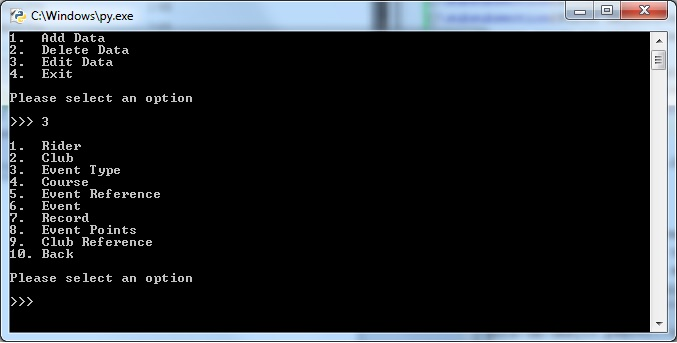
\includegraphics[width=\textwidth]{./Evaluation/CLI/CLI.jpg}
    \caption{The CLI Edit Interface} \label{fig:EditCLIEvid}
\end{figure}

\subsection{Core Objectives}
\subsubsection{First Objective}
The program needs to be able to calculate times and apply the points and positions for Team Cambridge specific competitions.
\subsubsection{Objective Completed?}

\subsubsection{Evidence}

\subsubsection{Second Objective}
The program needs to be able to upload the data to the Team Cambridge website.
\subsubsection{Objective Completed?}
This objective should be compleated however some modifation to the website may need to be done for it to proaply support the new database sturture.
\subsubsection{Evidence}

\subsection{Other Objectives}
\subsubsection{First Objective}
To retain the current results database.
\subsubsection{Objective Completed?}
The current database sould be able ot be manulay entered in to the databse, ohwever a tool to import the current database may be needed due to the size of the current database
\subsubsection{Evidence}

\subsubsection{Second Objective}
If I have enough time, to have the database being run off Network Attached Storage.
\subsubsection{Objective Completed?}
This objective has not been compleated due to time ristrictions.

\subsubsection{Thrid Objective}
If I have enough Time, to have a web interface that allows users to remotely access the database and upload results.
\subsubsection{Objective Completed?}
This objective has not been compleated due to time restriction.

\subsection{Objective Evaluation}

\section{Effectiveness}

%include as many subsections as necessary for your objectives
\subsection{Objective Evaluation}

\section{Learnability}

\section{Usability}

\section{Maintainability}

\section{Suggestions for Improvement}
I would like to patch the current programe to finish the core funtionalty in the main application and also bugfix the applicaiton so that it works as expected. The objective that were time dependent and were not implemented I would like to add and I feel that an import and export funtion would be useful to my client.
\section{End User Evidence}

\subsection{Questionnaires}

\subsection{Graphs}

\subsection{Written Statements}
